\chapter{Deep Learning: Modern Apporaches for Unsupervised Sentiment Analysis}\label{chapter:modernapproach}
We have just discussed some of the most recent work in the field of deep learning. In ~\autoref{chapter:wordrepresentation} we make use of them in unique ways and target a specific variant of sentiment analysis problem. Before that, we present some of the novel work done in this area ordered year-wise, which use various deep learning algorithms and in some way describe how the area has graduated over the years. 
\section{RNTN : Recursive Neural Tensor Networks}

\begin{figure}[ht!]
	\centering
		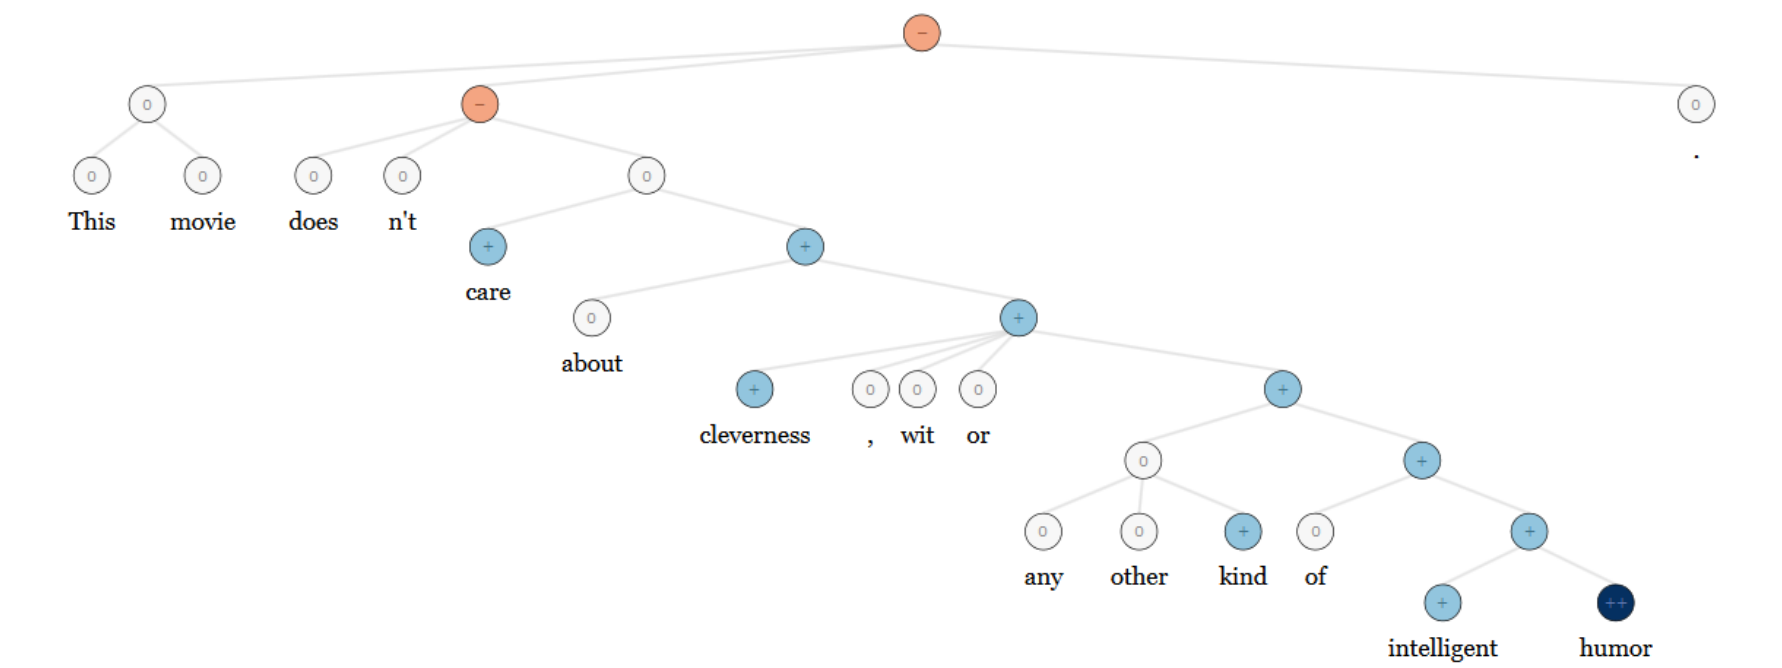
\includegraphics[height=40mm,  width=140mm]{figures/5_rntn.png}
		\caption[Example of Recursive Neural Tensor Network]{Example of Recursive Neural Tensor Network predicting sentiment at each node and capturing negation.}
			\label{rntn}
\end{figure}

Socher et. al~\parencite{rntnsocher} in 2013, introduced Recursive Neural Tensor Networks (RNTN) ~\autoref{rntn} and applied them to sentences and phrases of movie reviews and predicted sentiment across five broad categories in fine grained scheme (positive, slightly positive, neutral, negative and slightly negative) and across three categories in coarse grained scheme (positive, negative and neutral). The model was trained on a Sentiment Tree-bank which included fine grained sentiment labels for 215,154 phrases in the parse trees of the 11,855 sentences.  The inspiration behind the work is understanding compositionality in sentences using deep learning and leveraging it to identify sentiment.
\newline

\begin{figure}[ht!]
	\centering
		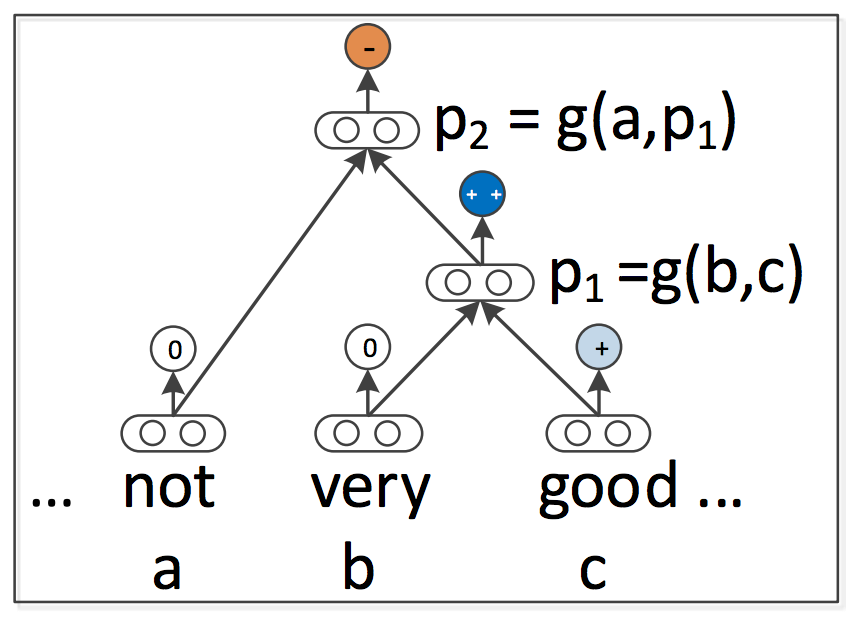
\includegraphics[height=40mm,  width=70mm]{figures/5_rnn.png}
		\caption[Recursive Neural Network Approach]{Recursive Neural Network models for sentiment: Computing parent vectors in a bottom up fashion using compositionality function \textbf{g}.}
			\label{rnn}
\end{figure}

RNTN are based on recursive neural network models.  They compute compositional vector representations for phrases of variable length and syntactic type. When n-gram is given as input to compositional models, it is parsed into a binary tree and each leaf node, corresponding to a word is represented as a vector. RNN then compute parent vectors in a bottom up fashion using the various composiitonality functions g. They are again given as input features to a classifier. ~\autoref{rnn} shows a tri-gram example.

Each vector is represented as a d - dimensional vector. They are first initialized randomly from a uniform distribution U( -r, r ), where r = 0.0001. They are then stacked in a word embedding matrix $L \in {R}_{d x |V|}$, where V is vocabulary size. L matrix is seen as a parameter which is trained jointly with the compositional models. For classification into five sentiment classes, the vectors can be fed to a softmax classifier. We compute the posterior probability over labels given the word vector via:

\begin{equation}
{y}_{\alpha} = softmax({W}_{s}a)
\end{equation}

Here, ${W}_{s}$ is sentiment classification matrix. This is repeated in the trigram for b and c as well.~\autoref{rnn}. There are other  models which are used to determine hidden layers / units. They are simple RNN ~\parencite{gollkuch} ~\parencite{socherrnn} and Matrix Vector RNN (MV-RNN)~\parencite{mvrnn}, which have also been proposed but RNTN tries to answer the quesion, which was unanswered by the latter two models, \textit{i.e.,} \textit{Can a single, more powerful composition function perform better and compose aggregate meaning from smaller constituents more accurately than many input specific ones?} And thus, the main idea behind RNTN is to use the same tensor based composition function, for all nodes. 

\begin{figure}[ht!]
	\centering
		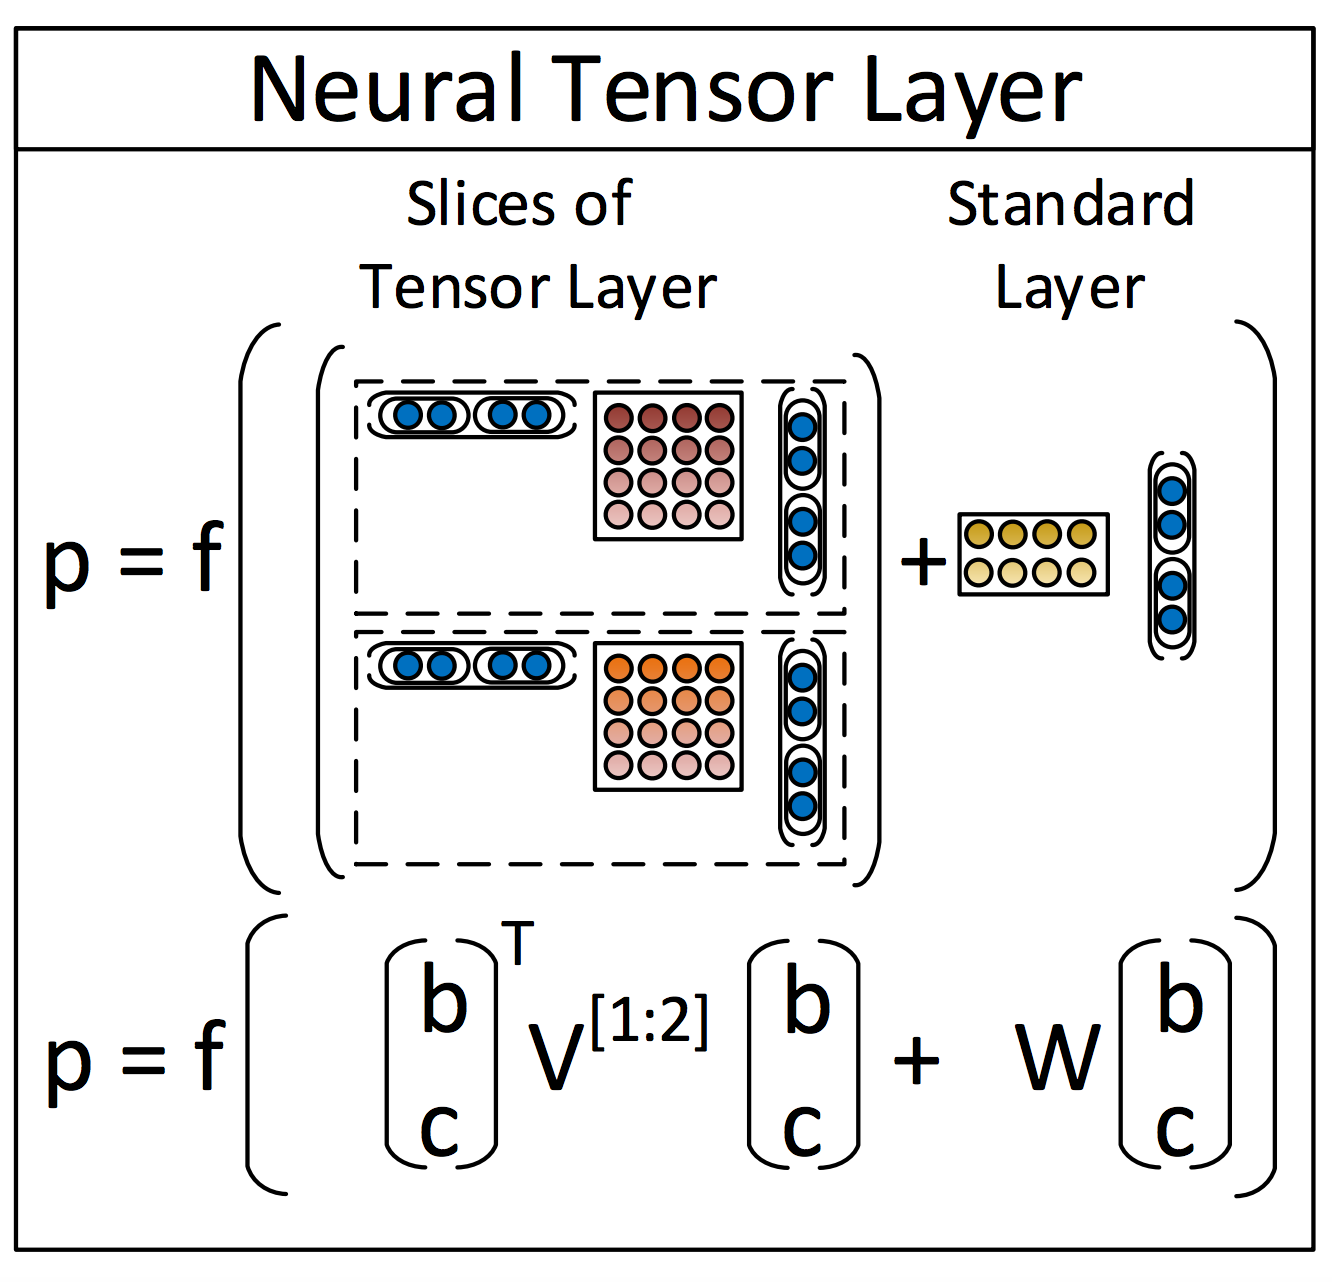
\includegraphics[height=60mm,  width=70mm]{figures/5_rntnmodel.png}
		\caption[Recursive Neural Tensor Network Layer]{Single layer of the Recursive Neural Tensor Network. Each dashed box represents one of d-many slices and can capture a type of influence a child can have on its parent}
			\label{rntnlayer}
\end{figure}
~\autoref{rntnlayer} shows a single layer neural network. An output of a tensor product h is defined as:

\begin{equation}
h =  {\begin{bmatrix}b \\c \end{bmatrix}}^{T} {V}_{[1:d]} \begin{bmatrix}b \\c \end{bmatrix};
\end{equation}

where, ${V}_{[1:d]}$ tensor defines multiple bi-linear forms.
Thus, to compute ${p}_{1}$, RNTN follows:


\begin{equation}
{p}_{1} = f ({\begin{bmatrix}b \\c \end{bmatrix}}^{T} {V}_{[1:d]} \begin{bmatrix}b \\c \end{bmatrix} + W \begin{bmatrix}b \\c \end{bmatrix})
\end{equation}
and similarly, ${p}_{2}$ is defined as:

\begin{equation}
{p}_{2} = f ({\begin{bmatrix}a \\{p}_{1} \end{bmatrix}}^{T} {V}_{[1:d]} \begin{bmatrix}a \\{p}_{1} \end{bmatrix} + W \begin{bmatrix}a \\{p}_{1} \end{bmatrix})
\end{equation}

Intuitively, we find that the RNTN slice tensor model, captures a specific type of composition.

\section{CNN : Convolutional Neural Networks}
Convolutional neural networks were originally designed for the application in Computer Vision by  Le Cunn et. al in 1998~\parencite{lecunoriginal}. But, they have shown promising results in several NLP tasks. In this work, Yoon Kim in 2014~\parencite{cnnsentence}, uses pre-trained word vectors along with CNN for several sentiment classification tasks. It was reported that the system performed exceedingly well, using a simple model with little hyper-parameter tuning.

\begin{figure}[ht!]
	\centering
		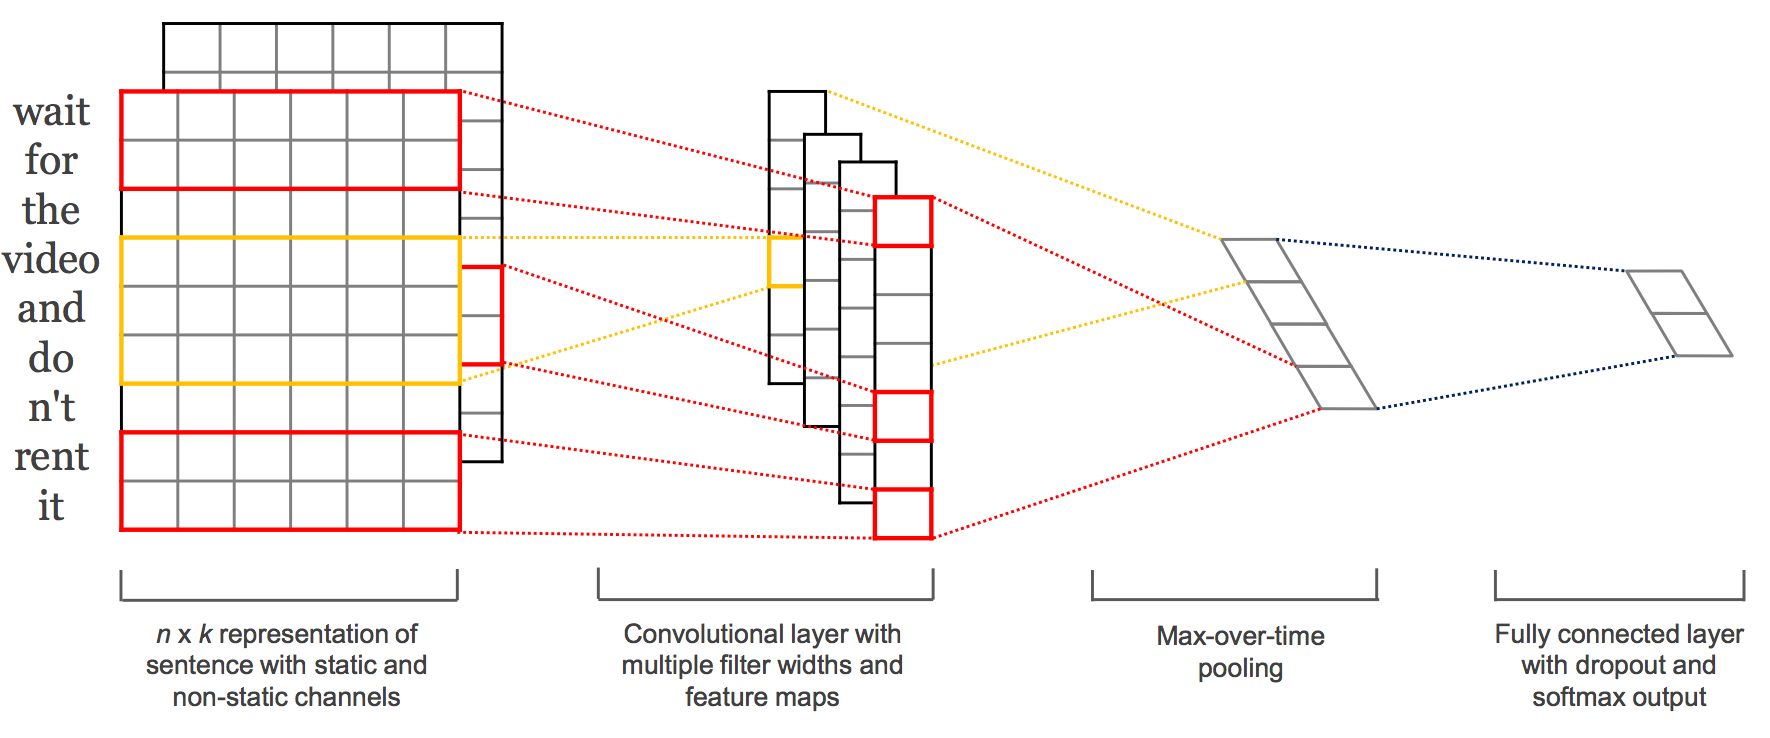
\includegraphics[height=50mm,  width=110mm]{figures/5_cnnsentence.png}
		\caption[CNN Model Architecture]{CNN Model architecture with two channels for an example sentence}
			\label{cnnsentence}
\end{figure}


We start with the model architecture~\autoref{cnnsentence}, ${x}_{i}$, a \textit{k} dimensional vector for i-th word in the sentence. A sentence of length n (padding if less than n) is represented as:

\begin{equation}
{x}_{1:n} = {x}_{1}  \oplus {x}_{2} \oplus  \cdots \oplus {x}_{n}
\end{equation}

$\oplus$ is the concatenation operator. In general, for a given concatenation of words: ${x}_{i:i+j}$, a convolutional operation involves application of a \textit{filter} w over a window of h words producing a new feature ${c}_{i}$:

\begin{equation}
{c}_{i} = f(w. {x}_{i:i+h-1} + b)
\end{equation}

where b is the bias term and f is a non linear function such as hyperbolic tangent. This filter is then applied to each possible window to produce a \textit{feature map}.

\begin{equation}
c = [{c}_{1}, {c}_{2}, \cdots , {c}_{n-h+1}]
\end{equation}

We then apply the maximum -over time pooling operation~\parencite{nlpscratch} to c and choose the maximum value, $\hat{c} = max{c}$ as the feature corresponding to this particular filter. This helps to capture the most important feature per feature map. Overall, the model uses many filters to obtain multiple features. These features form the pen-ultimate layer and they are then fed to a full connected soft-max classifier layer , which outputs the probability distribution over sentence class labels. 

Also for regularization, a dropout was implemented on the pen-ultimate layer with constraint on l-2 normalization of weight vectors. It helps prevent co-adaptation of hidden units. For the purpose, a proportion  of the hidden units are dropped out or set to zero during forward back propagation step. Or given the penultimate layer of max-pooled features, with m filters: z =   $[ \hat{{c}}_{1} , \cdots , \hat{{c}}_{m} ]$, instead of using

\begin{equation}
 y = w . z + b
\end{equation}

The output unit \textit{y} in forward propagation dropout uses

\begin{equation}
 y = w .( z \circ  r) + b
\end{equation}

Where, $\circ$ is the element-wise multiplication operator and r is the masking vector of Bernouli random variables with probability p of being 1. Gradients are forward propagated through the unmasked units. And during test time, the weights are scaled up by a factor of \textit{p}, such that $\hat{w} = pw$ and $\hat{w}$ is used to score unseen sentences. Also, a re-scaling of w using l2 normalization is also performed.

\section{LSTM : Long and Short Term Memory Networks}
\begin{figure}[ht!]
	\centering
		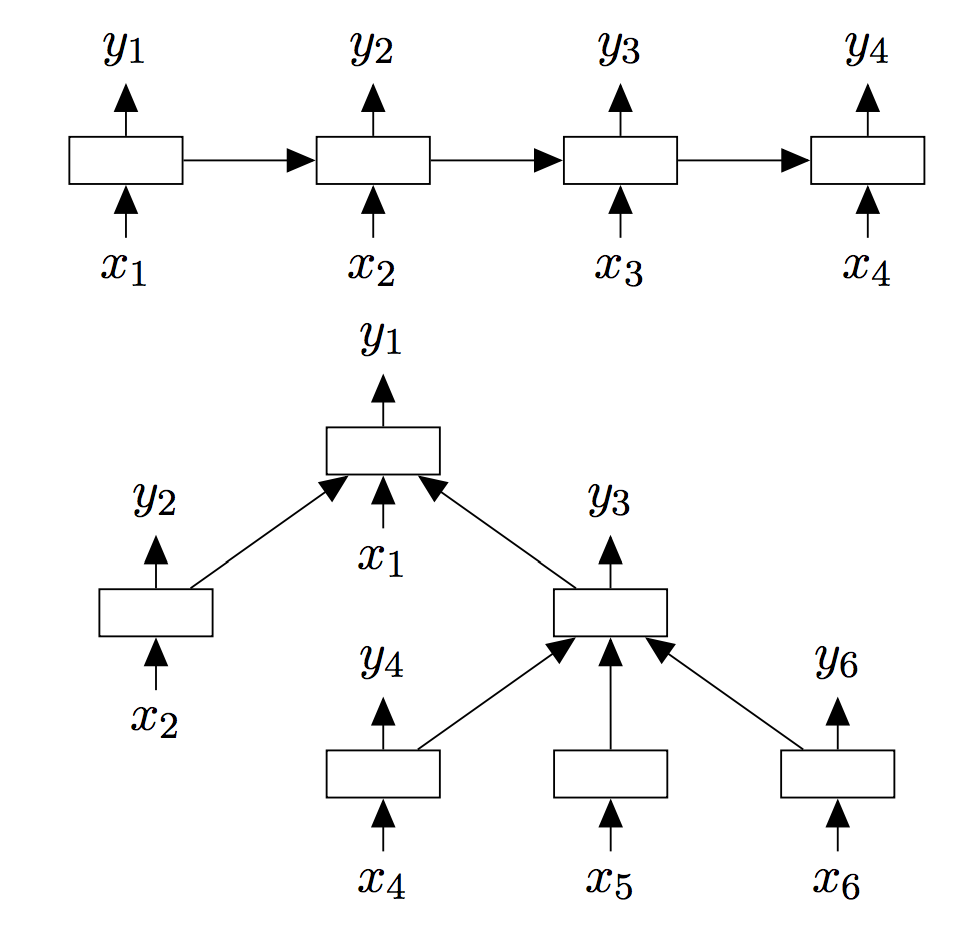
\includegraphics[height=65mm,  width=70mm]{figures/5_lstm1.png}
		\caption[LSTM Structures]{\textbf{Top:} Chain Structured LSTM;\textbf{ Bottom:} Tree-Structured LSTM}
			\label{lstmstructure}
\end{figure}

LSTM's or Long and Short Term Memory network is a type of recurrent neural network architecture, which have shown extremely good results on sequence modeling tasks. They were first introduced by Sepp Hochreiter and Schmidhuber Jurgen in 1997 ~\parencite{lstmoriginal}. In 2015, Kai et. al ~\parencite{lstmsentiment} propose Tree-LSTM, a generalization of LSTMs to tree structured network topologies~\autoref{lstmstructure}.They are inspired to model the view, to combine the words into phrases as in natural language. Tree structured LSTM's are currently out-performing all the baselines for semantic relatedness task and sentiment classification task.
\newline

The problem found out, in the RNN application over long distance sequence modeling is that during training time, the gradient vector components can grow or decay exponentially over long sequences. This problem is commonly known as vanishing or exploding gradient. This makes it difficult for an RNN model to learn long distance co-relations in a sequence.  LSTMs address this problem, by introducing a \textbf{memory cell}. The task of a memory cell is to preserve states over long periods of time. 

Kai, et. al ~\parencite{lstmsentiment}  provides the two extensions to the basic LSTM structure: the \textit{Child-Sum Tree-LSTM} and \textit{N-ary Tree-LSTM}. Both variants allow for richer network topologies, where each LSTM units can incorporate information from multiple child units.

Each Tree LSTM unit consists of input and output gates ${i}_{j}$ and ${o}_{j}$ a memory cell ${c}_{j}$ and hidden cell ${h}_{j}$. The updates of the gating vector depends on several child units. Instead of a single forget fate, a Tree-LSTM unit consists of one forget gate ${f}_{jk}$ per child unit \textit{k}. This allows for selectivity of information from each child. Each Tree Structured LSTM takes a word vector ${x}_{j}$ as input vector. The input word at each node depends on the tree structure used for the network. For a dependency tree based LSTM, each node in tree takes the head word as the input, whereas, for constituency tree, the leaf node take the corresponding word vector as input.

Given a tree, C(j) are set of children of node j. Thus, transition equations for \textbf{Child-Sum Tree LSTM} and $k \in {C}_{j}$ are: 

\begin{equation}
{\tilde{h}}_{j} =  \sum_{k \in C(j)} {h}_{k} 
\end{equation}

\begin{equation}
{i}_{j} = \sigma  \big(   {W}^{(i)} {x}_{j} + {U}^{(i)} {\tilde{h}}_{j} +    {b}^{(i)}   \big)  
\end{equation}

\begin{equation}
{f}_{jk} = \sigma  \big(   {W}^{(f)} {x}_{j} + {U}^{(f)} {h}_{k} +    {b}^{(f)}   \big)  
\end{equation}

\begin{equation}
{o}_{j} = \sigma  \big(   {W}^{(o)} {x}_{j} + {U}^{(o)} {\tilde{h}}_{j} +    {b}^{(o)}   \big)  
\end{equation}

\begin{equation}
{u}_{j} = \tanh  \big(   {W}^{(u)} {x}_{j} + {U}^{(u)} {\tilde{h}}_{j} +    {b}^{(u)}   \big)  
\end{equation}

\begin{equation}
{c}_{j} = {i}_{j}  \odot  {u}_{j} +  \sum_{k \in C(j)} {f}_{jk}  \odot   {c}_{k}    
\end{equation}

\begin{equation}
{h}_{j} = {o}_{j} \tanh {c}_{j}    
\end{equation}


Intuitively,  the parameter matrix in above equations can be treated as encoding correlations between the component vectors of the Tree-LSTM unit, the input ${x}_{j}$ , and the hidden states ${h}_{k}$ of the unit’s children. Child-sum LSTM's are well suited for trees whose branching factor is high, or whose children are un-ordered. Thus, it's a good choice for a dependency trees.

On the other hand N-ary Trees (not discussed in detail here), are good where the branching factor is known and at most \textit{N} or the children are ordered. 

The sentiment classification models using Tree LSTM models aim to predict labels $\hat{y}$ from a set of classes $y$ for some subset of nodes in tree. For example: Phrase spanned by the node. At each node j, thelabel ${\hat{y}}_{j}$ given the input ${\{x\}}_{j}$  observed at nodes in the subtree rooted at j is predicted by a softmax classifier that takes one hidden state ${h}_{j}$ at the node as the input:
\begin{equation}
{\hat{p}}_{\theta} ( y | {\{x\}}_{j}  ) = softmax  \big(  {W}^{(s)} {h}_{j} + {b}^{s}  \big)
\end{equation}
\begin{equation}
{\hat{y}}_{j} = \operatorname*{arg\,max}_y  {\hat{p}}_{\theta} ( y | {\{x\}}_{j}  )
\end{equation}
The cost function is then the negative log-likelihood of the true class labels ${y}^{(k)}$ at each labeled node.
\begin{equation}
J(\theta) = -\frac{1}{m}  \sum_{k=1}^{m} log {\hat{p}}_{\theta} \big(  {y}^{(k)} | {\{x\}}^{k}\big) + \frac{\lambda}{2}  {\parallel \theta \parallel}_{2}^{2}    
\end{equation}
where, \textit{m} is the number of labeled nodes in the training set and \textit{k} indicates the k-th labeled node.
\section{Comparative Evaluation}
The current state of the art for fine grained or five class sentiment classification is with Tree based LSTM as discussed above. In the paper ~\parencite{lstmsentiment}, the authors provide a comparative evaluation of all the methods which were state of the arts over a period of time, few of which have also been covered in current literature. 
\newline


The data-set used for evaluation is the \textbf{Stanford Sentiment Treebank} ~\parencite{rntnsocher} and the experiments are conducted on two types of categories, \textbf{Fine-grained} implies classification over five classes, positive, negative, slightly positive, slightly negative and neutral and binary or coarse grained implies positive and negative sentiment classes. As, we can see in the ~\autoref{compareeval} the current benchmark for the fine grained category is 50.6\% obtained by the Constituency Tree LSTM with tuning. Whereas, the model proposed by Kim et. al~\parencite{cnnsentence} achieves the state of the art in overall binary classification with 88.1\% accuracy over test data.  

\begin{figure}[ht!]
	\centering
		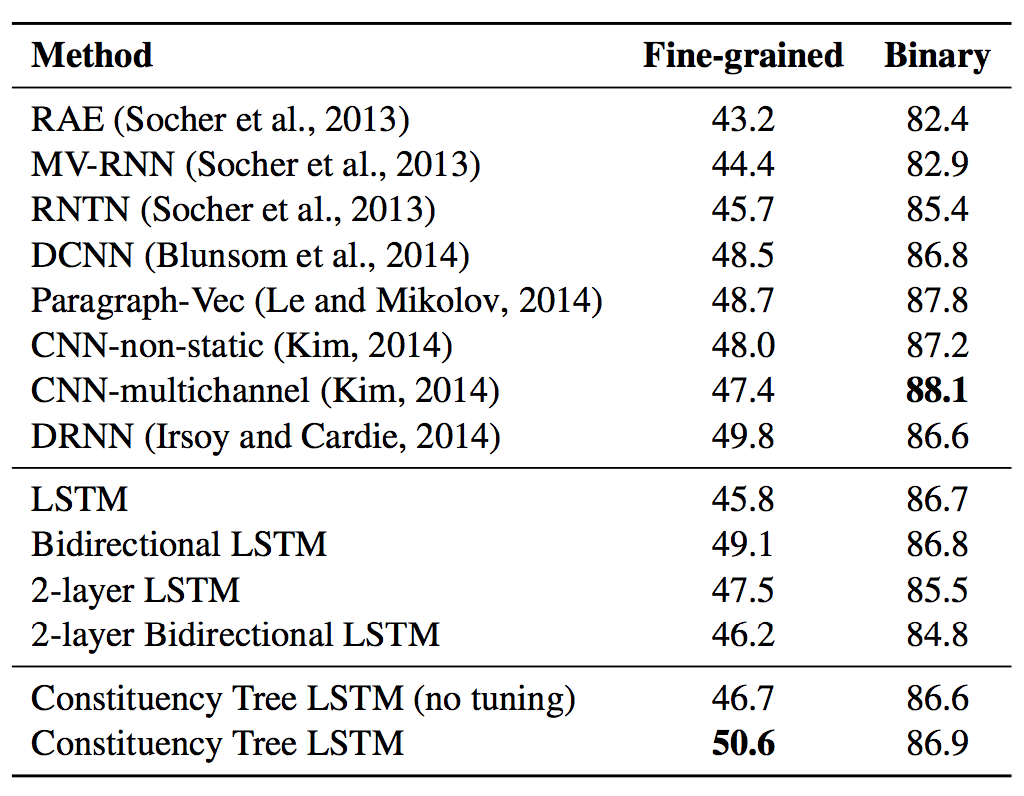
\includegraphics[height=55mm,  width=65mm]{figures/5_comparativeevaluation.png}
		\caption[Comparative Evaluation]{Test set accuracies on Stanford Sentiment Tree-bank Dataset.}
			\label{compareeval}
\end{figure}


